% Chapter 1

\chapter{Introducción general} % Main chapter title

\label{Chapter1} % For referencing the chapter elsewhere, use \ref{Chapter1} 
\label{IntroGeneral}

%----------------------------------------------------------------------------------------

% Define some commands to keep the formatting separated from the content 
\newcommand{\keyword}[1]{\textbf{#1}}
\newcommand{\tabhead}[1]{\textbf{#1}}
\newcommand{\code}[1]{\texttt{#1}}
\newcommand{\file}[1]{\texttt{\bfseries#1}}
\newcommand{\option}[1]{\texttt{\itshape#1}}
\newcommand{\grados}{$^{\circ}$}

%----------------------------------------------------------------------------------------

%\section{Introducción}

%----------------------------------------------------------------------------------------

En este capítulo se presenta la problemática y la motivación que llevaron a la realización del presente trabajo.

\section{Descripción de la problemática}

La fenómica hace referencia a la obtención de un gran caudal de datos de las características de las plantas, lo que se denomina el fenotipo de la planta. Esta disciplina está en auge en la actualidad debido a sus aplicaciones potenciales. Por un lado, habilita el mejoramiento a gran escala debido a que es necesario vincular una gran cantidad de datos genéticos con datos fenotípicos para identificar la función de los genes. Por otro lado, si se incluyen otros conjuntos de datos como son los climáticos, permite realizar predicciones precisas sobre el comportamiento de las variedades, el cual es necesario para implementar lo que se conoce como agricultura de precisión. Sin embargo, la fruticultura no ha dado el salto hacia la fenómica.

En la  Estación Experimental Agropecuaria (EEA) de San Pedro se ha logrado secuenciar el ADN de más de 250 variedades de duraznero \cite{ARTICLE:1} disponiendo de una base de datos genómica de 75 gigabases (Gb) de ADN. Esta base permite identificar genes que controlan características del duraznero mediante algoritmos de inteligencia artificial (IA). Además, se dispone de datos climáticos diarios que se toman de forma automática que incluyen: las temperaturas medias, precipitaciones, horas de frío, radiación, etc. Esta información se combina con los datos genómicos y posteriormente, con modelos de IA se predice el comportamiento de las variedades en escenarios climáticos futuros.

En la actualidad, las heladas primaverales son el mayor problema de los frutales a nivel mundial. Este fenómeno ocurre cuando las flores abiertas se someten a temperaturas cercanas a los -2.5 °C. Las heladas primaverales, tienen una temparatura parecida a cualquier otra helada que se puede presentar en la temporada de invierno. Sin embargo, estas heladas suelen presentarse despues del invierno, creando un gran impacto contra las flores y los frutos de los frutales. Los productores de frutas en general, se ven altamente afectados pagando un alto precio por estas inesperadas heladas tardías. En la figura \ref{fig:helada}, se puede observar como este fenomeno meteorológico afecta a los frutales.

\begin{figure}[htpb]
	\centering
	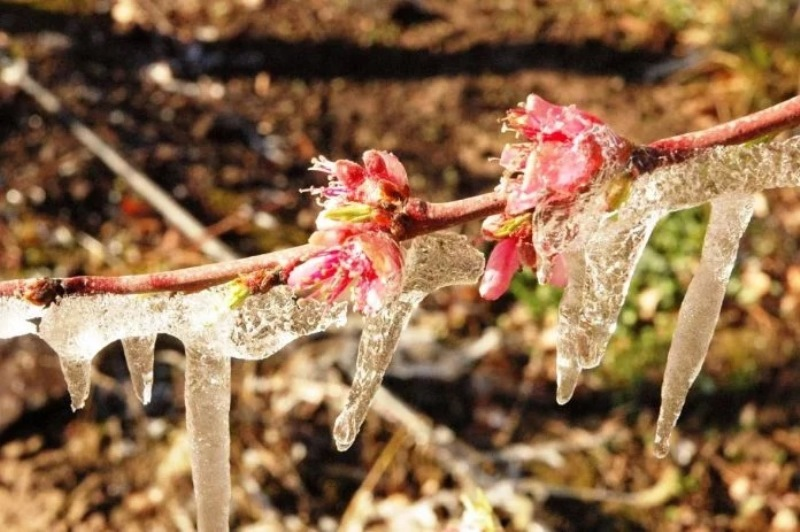
\includegraphics[scale=.5]{./Figures/heladas3.jpeg}
	\caption{Frutales afectados por las heladas primaverales \cite{WEBSITE:1}.}
	\label{fig:helada}
\end{figure}

\section{Motivación}

Por este motivo, es del interés del Instituto Nacional de Tecnología Agropecuaria (INTA) determinar el estado fenológico a campo y mejorar para la tolerancia a heladas.

Para determinar el estado fenológico a campo, es necesario conocer el número de flores que se encuentran en estado vulnerable ante un pronóstico de heladas primaverales, así también como la densidad de flores.

En cuanto al mejoramiento, se ha realizado una caracterización a gran escala de la tolerancia a heladas de la colección de duraznero con el objetivo de identificar los genes responsables. Parte de ese experimento consistió en determinar en registrar el estado fenológico mediante fotos.

El presente trabajo permitirá automatizar la toma de datos de varetas de duraznero, a partir de fotos para aumentar el caudal de datos y mejorar los modelos de IA.

\section{Requerimientos}

\begin{enumerate}
	\item Requerimientos funcionales
		\begin{enumerate}
			\item El sistema tomará como entrada imágenes de varetas de durazneros en formato JPG.			
			\item El algoritmo debe detectar la presencia de las varetas de los durazneros e identificar el tipo de flor que posee.			        
			\item El algoritmo debe identificar el estado fenológico de cada flor de duraznero en la vareta. Este estado puede ser F de flor abierta, E de flor cerrada o G de flor sin pétalos. 
			\item El algoritmo debe determinar la cantidad de flores por centímetro de vareta.
			\item El sistema debe entregar como resultado un archivo en formato JSON con los datos detectados por el algoritmo y una imagen donde se puedan visualizar las detecciones.
			\item El sistema debe funcionar en una computadora local.
		\end{enumerate}
	\item Requerimientos de diseño e implementación
		\begin{enumerate}
			\item El diseño debe ser modular.
			\item El algoritmo se elaborará en una notebook de Google Colab, utilizando el lenguaje de  programación Python y bibliotecas de IA correspondientes. 
		\end{enumerate}
	\item Requerimiento de evaluación y prueba
	\begin{enumerate}
			\item El modelo se evaluará con imágenes provenientes del mismo dataset de imágenes entregado por el cliente.
			 \item Las métricas que se utilizarán para la evaluación del modelo serán: \textit{mean average precision} (mAP), matriz de confusión, \textit{precision}, \textit{recall}, \textit{F1}, \textit{accuracy}.
		\end{enumerate}
	\item Requerimientos de documentación
	\begin{enumerate}
			\item El funcionamiento del sistema debe estar correctamente explicado y documentado.
			 \item El código en la notebook estará correctamente comentado como parte de buenas prácticas del desarrollo de software.
			 \item Inclusión de documentación en un repositorio, mediante un archivo README.md (opcional).
		\end{enumerate}
\end{enumerate}

\section{Objetivo y alcances}

El objetivo de este trabajo es desarrollar un algoritmo que permita automatizar la toma de datos de las flores de duraznero a través de fotos de varetas.

El presente trabajo incluye:
\begin{itemize}
	\item El preprocesamiento de las fotos para entrenar el modelo.
	\item La selección del modelo a entrenar.
	\item La elaboración del notebook de pruebas en Python.
	\item La implementación local del modelo.
\end{itemize}

El trabajo no incluye:
\begin{itemize}
	\item La recolección de datos/fotos.
	\item La integración con otros modelos que utilice el cliente.
\end{itemize}


%----------------------------------------------------------------------------------------

\section{Estado del arte}

Si estás familiarizado con \LaTeX{}, entonces podés explorar la estructura de directorios de esta plantilla y proceder a personalizarla agregando tu información en el bloque \emph{INFORMACIÓN DE LA PORTADA} en el archivo \file{memoria.tex}.  

Se puede continuar luego modificando el resto de los archivos siguiendo los lineamientos que se describen en la sección \ref{sec:FillingFile} en la página \pageref{sec:FillingFile}.

Debés asegurarte de leer el capítulo \ref{Chapter2} acerca de las convenciones utilizadas para las Memoria de los Trabajos Finales de la \degreename.

Si sos nuevo en \LaTeX{}, se recomienda que continúes leyendo el documento ya que contiene información básica para aprovechar el potencial de esta herramienta.


%----------------------------------------------------------------------------------------

